\cotefile{156-8}
\scanpage{10}
\mspage{\unsure{1bis|bis}}
% archive sheet number: 10
\margin{27 juin}
% slanted

Avant de passer aux figures, il faudrait donner quelques compléments aux \unsure{$M$} liminaires

\deleted{\uline{Prop} Si $Y\overset{\circ}{\ll}X$ et $Y\overset{\unsure{\circ}}{\ll}X'$ alors $X\unsure{\gtrless|\bowtie}$}

\deleted{\uline{Prop} Supposons $X\gtrless Y$. Si $Z\overset{\circ}{\ll}X$, alors \unsure{$\ll$}}
\[
\deleted{Z\ll\unsure{Y}\ \Longleftrightarrow\ \unsure{X}\ll\unsure{Y}}
\]
\deleted{\uline{Dém} $\Longleftarrow$ \unsure{trivial}, prouvons $\Longrightarrow$. Par $\unsure{\mathrm{Mog}|\mathrm{Mag}}\,2$, $\exists\,Y'$ \unsure{avec}}
\[
\deleted{Z\overset{\circ}{\ll}Y'\leq Y}
\]
\noindent\fbox{\parbox{.94\linewidth}{\uline{Prop 1} \unsure{Si} $X'\leq X$, $Y'\leq Y$, alors $X\gtrless Y\Longrightarrow X'\gtrless Y'$}}

\uline{Prop 1.} a) $X\gtrless Y$ est symétrique et réflexive

b) Si $X'\leq X$, $Y'\leq Y$, alors $X\gtrless Y\Longrightarrow X'\gtrless Y'$

\uuline{Dém.} a) \deleted{\unsure{symétrie}} trivial par \uuline{Mog 3 a)}.

b) Soit $X''\in\widetilde X'\setminus\widetilde X'\cap\widetilde Y'$, $Y''\in\widetilde Y'\setminus\widetilde X'\cap\widetilde Y'$. \inserted{A prouver $X''\mathrel{|\unsure{\circ|0}|}Y''$.} Si $X'',Y''\notin\widetilde X\cap\widetilde Y$, alors $X''\mathrel{|\circ|}Y''$ par déf de $X\gtrless Y$. Si $X''\in\widetilde X\cap\widetilde Y$, on a $X''\in\widetilde Y$, $Y''\in\widetilde Y'\subset\widetilde Y$, d'autre part évidemment $X''\neq Y''$, donc $X''\mathrel{|\circ|}Y''$ par \uuline{Mog 4}.

\margin{\uline{Prop. 2.} Si $X\gtrless Y$, alors $X\mathrel{|\circ|}Y\Longleftrightarrow X\neq Y$. \uuline{dém} $\Longrightarrow$ par Mog 3 a). Inv. supp. $X\neq Y$, \deleted{\unsure{et}} si $X\nleq Y$ et $Y\nleq X$, i.e. $X\notin\widetilde X\cap\widetilde Y$, $Y\notin\widetilde X\cap\widetilde Y$, on a $X\mathrel{|\circ|}Y$ par déf. de $X\gtrless Y$. Si $X\leq Y$, ou $Y\leq X$, on applique \uline{Mog 4}}
% margin note written sideways

\deleted{\uline{Prop \unsure{2}}}\inserted{\uline{Cor 1}} Soient $X,Y$ avec $X\gtrless Y$. Soit $Z$ \unsure{avec} $Z\overset{\circ}{\ll}X$.

Alors
\[
Z\ll Y\ \Longleftrightarrow\ \deleted{Z}X\leq Y
\]

Énonçons tout de suite corollaire

\uline{Corollaire 2} Si $Z\overset{\circ}{\ll}X$, $Z\overset{\circ}{\ll}Y$, et si $X\gtrless Y$, alors $X=Y$.

En effet, on a $X\ll Y$ et $Y\ll X$, donc $X=Y$ par \uline{Mog 1 a}.

Prouvons \deleted{\uline{Prop 2}}\inserted{cor 1}. $\Longleftarrow$ évident, prouvons
\[
Z\overset{\circ}{\ll}X,\ Z\ll Y\ \Longrightarrow\ X\ll Y\qquad(\text{si }X\gtrless Y).
\]
\deleted{\unsure{Soit}} Par \uuline{Mog 2}, $\exists\,Y'$ \unsure{avec} $Z\overset{\circ}{\ll}Y'\leq Y$, par prop $1$ on a $X\gtrless Y'$, il suffit de prouver $X=Y'$ (d'où $\underset{\inserted{\substack{\Vert\\Y'}}}{X}\leq Y$), i.e. on est ramené au cas du cor. Mais si on avait $X\neq Y$

\[
\boxed{Z\overset{\circ}{\ll}X,\ Z\overset{\circ}{\ll}Y,\ X\gtrless Y\ \Longrightarrow\ X=Y.}\quad\deleted{\unsure{Cor}}
\]

\deleted{\unsure{Prouvons} $Z\unsure{\notin|\in}\widetilde X\cap\widetilde Y$, \unsure{on a}}
\margin{\deleted{$Z\in\widetilde X\setminus\widetilde X\cap\widetilde Y$ \unsure{?}}}

\deleted{\deleted{$Z\in$} Il suffit de prouver $X\neq Y$ (car on a de même $Y\leq X$). on aurait $\widetilde X\subset\widetilde Y$, \deleted{sinon} \unsure{on|ou} aurait $\widetilde X\in\widetilde X\cap\widetilde Y$. Sinon, on aurait $X\mathrel{|\circ|}Y$ (cf lemme), \deleted{d'où} et comme $Z\overset{\circ}{\ll}X$, $Z\overset{\circ}{\ll}Y$ on conclurait $Z\mathrel{|\circ|}Z$ par Mog 3 b), absurde par Mog 3 a). \unsure{Ainsi}}

on aurait par prop 2 $X\mathrel{|\circ|}Y$, donc $Z\mathrel{|\circ|}Z$ par Mog 3 b), absurde par Mog 3 a).

\scanpage{11}
\mspage{2bis}
% archive sheet number: 11

\uline{Cor. 3} Soit $X\unsure{\gtrless|\bowtie}Y$. Alors
\[
X\unsure{\,\cdot\,}\ll Y\ \Longleftrightarrow\ X\leq Y
\]
\deleted{En effet,} On applique cor 1 avec $Z=X$.

\uline{Proposition 3.} \deleted{Supposons} $X\overset{\circ}{\ll}Y\overset{\circ}{\ll}Z$ \deleted{$\unsure{\Longleftrightarrow}$}\inserted{implique} $X\overset{\circ}{\ll}Z$.
\[
\deleted{\Longleftrightarrow\ X\overset{\circ}{\ll}Y\text{ et }Y\overset{\circ}{\ll}Z}
\]
\deleted{a) Supposons $X\overset{\circ}{\ll}Y$ et $Y\overset{\circ}{\ll}Z$, prouvons $X\overset{\circ}{\ll}Z$, i.e. $X\ll Z'\leq Z\Longrightarrow Z'=Z$. \unsure{Comme}}

Par $\unsure{\mathrm{Mog}|\mathrm{Mag}}\,2$ $\exists\,Z'$ \unsure{avec} $X\overset{\circ}{\ll}Z'\leq Z$, \deleted{\unsure{on a|où}} \deleted{\unsure{par Mog}} prouvons $Z'=Z$. Sinon, par Mog 4 on aurait $Z'\mathrel{|\unsure{\circ|0}|}Z$, et par Mog 3 b) $X\mathrel{|\circ|}Z$, d'autre part

\diagram{\begin{tikzcd}[ampersand replacement=\&,column sep=small,row sep=small]
X\arrow[r,phantom,"\overset{\circ}{\ll}"{description}]\arrow[dr,phantom,"\overset{\circ}{\ll}"{description,rotate=-45}]\&Y\arrow[r,phantom,"\overset{\circ}{\ll}"{description}]\&Z\arrow[dl,phantom,"\leq"{description,rotate=45}]\\
\&Z'\&
\end{tikzcd}}

par Mog 3 b) cela implique $X\mathrel{|\circ|}Y$ puisque $Y\overset{\circ}{\ll}Z$, puis $X\mathrel{|\circ|}X$ puisque $X\overset{\circ}{\ll}Y$, \deleted{d'où $X\mid$} mais $X\mathrel{|\circ|}X$ contredit Mog 3 a).

\deleted{\unsure{b)}}\inserted{NB} Supposons \inserted{$X\ll Y\ll Z$ et} $X\overset{\circ}{\ll}Z$. Alors $Y\overset{\circ}{\ll}Z$, car si on avait $Y\ll Z'\unsure{<|\leq}Z$, on en conclurait $X\ll Z'<Z$, contrairement à $X\overset{\circ}{\ll}Z$. \deleted{\unsure{Prouvons}} \deleted{par} Mais on n'a pas \unsure{néc\textsuperscript{t}} $X\overset{\circ}{\ll}Y$, \unsure{exple}.

\figure{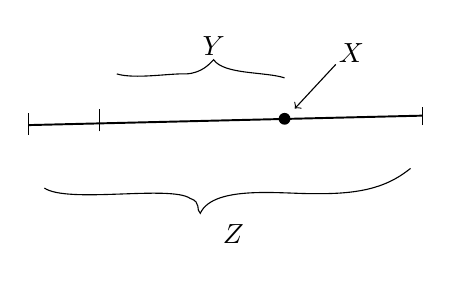
\begin{tikzpicture}[x=1cm,y=1cm]
\draw[line width=.7pt] (0,0)--(5,.12);
\draw (0,-.12)--(0,.15) (.9,-.08)--(.9,.2) (5,0)--(5,.23);
\fill (3.25,.08) circle (.075);
\draw (1.12,.65) .. controls (1.35,.58) and (1.8,.66) .. (2,.65) .. controls (2.2,.66) and (2.3,.78) .. (2.35,.83) .. controls (2.48,.64) and (3,.68) .. (3.25,.6);
\node at (2.35,1) {$Y$};
\draw[->] (3.9,.77)--(3.38,.21);
\node at (4.1,.91) {$X$};
\draw (.2,-.8) .. controls (.5,-1) and (1.8,-.76) .. (2.05,-.93) .. controls (2.2,-.98) and (2.12,-1.08) .. (2.18,-1.12) .. controls (2.35,-.75) and (3.25,-.88) .. (3.65,-.87) .. controls (4.3,-.88) and (4.6,-.75) .. (4.85,-.55);
\node at (2.6,-1.38) {$Z$};
\end{tikzpicture}}

\uline{Cas des figures}

\uline{Prop 1}.F a) $F\gtrless G$ sym. \unsure{réfl.}

b) $F\gtrless G$, $F'\leq F$, $G'\leq G\Longrightarrow F'\gtrless G'$

\uline{Prop \unsure{2|?}}.F Si $F\gtrless G$, \deleted{\unsure{Prop}} alors $F\ll G\Longleftrightarrow F\leq G$

\uline{Cor} Dans l'ens \unsure{de|des} $\unsure{\mathrm{Ssfig}(F)|\mathrm{Ssfi}_0(F)}$, $\ll$ et $\leq$ coïncident

\scanpage{12}
\mspage{3}
% archive sheet number: 12

\[
\begin{aligned}
F\parallel G&\Longleftrightarrow\ \forall\,X\in\widetilde F,Y\in\widetilde G,\ \text{on a }X\parallel Y\\
&\inserted{\Longleftrightarrow\ F\unsure{\gtrless|\bowtie}G\text{ et }F\cap G=\varnothing}
\end{aligned}
\]
On n'écrira $F\mathrel{|\unsure{\circ|0}|}G$ que si $F,G$ sont élémentaires, i.e. sont ``$\in M$'', idem pour $\overset{\circ}{\ll}$.

\deleted{\uline{Proposition} Soient $F,G\in\unsure{\mathfrak f|\mathscr F|\mathcal F|f}$, $L=F\cap G$, $F'\ll F$, $G'\ll G$,}

On a

\deleted{\unsure{cor}}

\uline{Proposition 1} Propriétés formelles de $\mathfrak f$, $\leq$ a) \unsure{distributivité} et b) en tant qu'ensemble de parties de $M$.

\margin{y inclus l'existence \unsure{conditionnée|conditionnelle} des Sup et \unsure{inconditionnée|inconditionnelle} des $\operatorname{Inf}_{I}$ ($I\neq\varnothing$)}
% slanted

\uline{Proposition 2} a) $F\gtrless G$, $F'\leq F$, $G'\leq G\Longrightarrow F'\gtrless G'$
\margin{``division'' de prop \unsure{1|1^{\circ}}.F \unsure{b)}}
% slanted

\deleted{b) $F\parallel G$, $F'\ll F$, $G'\ll G\Longrightarrow F'\parallel G'$}

\unsure{b)} \deleted{\unsure{En|Et}} Si $F=\bigcup_i F_i$ Sup de sous-figures, alors $G\gtrless F\unsure{\Longleftrightarrow}\forall i,\ G\gtrless F_i$.

Donc si $F=\bigcup F_i$, $G=\bigcup G_j$, $F\gtrless G$ ssi $\forall i,j,\ F_i\gtrless G_j$.

\margin{Prop 1, Prop 2 concernent $\leq$ seulement}
% slanted

\uline{Proposition 3} \deleted{Soient}\inserted{Soient} \deleted{$F,G$, $F\gtrless G$, \deleted{$F'\ll F$}, $L=F\cap G$, $F'\ll F$, $G'\ll G$,}

\diagram{\begin{tikzcd}[ampersand replacement=\&,column sep=small,row sep=small]
G\arrow[r,phantom,"\ll"{description}]\&F\arrow[d,phantom,"\leq"{description,rotate=90}]\\
\&F'
\end{tikzcd}} ,

alors $\exists\,G'$ \unsure{avec}
\[
\deleted{\unsure{\widetilde G}\cap\operatorname{Omb}(F')}
\]
\diagram{\begin{tikzcd}[ampersand replacement=\&,column sep=small,row sep=small]
G\arrow[r,phantom,"\ll"{description}]\arrow[d,phantom,"\leq"{description,rotate=90}]\&F\arrow[d,phantom,"\leq"{description,rotate=90}]\\
G'\arrow[r,phantom,"\ll"{description}]\&F'
\end{tikzcd}}
\[
G'=\operatorname{Inf}^{\ll}(F',G).
\]
On a
\[
\widetilde G'=\widetilde G\cap\operatorname{Omb}(F')
\]
Posant $G'=G_{F'}$ \inserted{ou $G(F')$} ou ${}^{F'}G$ \inserted{ou $F'|G$}, on a
\[
F'\longmapsto G_{F'}:\ \unsure{\mathrm{Ssfig}|\mathrm{Ssfi}_0}(F)\;\text{---}\;\mathrm{Ssfig}(G)
\]
\inserted{est croissant et} commute aux Sup et aux Inf quelconques.

\scanpage{13}
\mspage{4}
% archive sheet number: 13

\uline{Cor. 1} Si $G\leq F$, alors $G'=G\cap F'$ \inserted{(donc $\widetilde G'=\widetilde G\cap\widetilde F'$)}, i.e.
\[
\operatorname{Inf}^{\ll}(G,F')=\operatorname{Inf}^{\leq}(G,F')
\]
\uline{Cor. 2} (cf \unsure{haut} \unsure{verso|prop.} 5)

\uline{Prop 5} Soient $F,G$ avec $F\unsure{\gtrless|\bowtie}G$, \inserted{$L=F\cap G$,} $F'\ll F$, $G'\ll G$, d'où $F'_L\deleted{\ll}$, $G'_L\ll L$. Alors
\[
\deleted{\text{a)}\quad\unsure{F'_L}\gtrless G'_L\Longleftrightarrow}
\]
\[
\begin{aligned}
\text{a)}\quad F'\gtrless G'&\Longleftrightarrow F'_L\gtrless G'_L\\
\text{b)}\quad F'\parallel G'&\Longleftrightarrow F'_L\parallel G'_L
\end{aligned}
\]

\uline{Cor.} Si $F'_L=\varnothing$, alors $F'_{\deleted{L}}\parallel G'$ pour \unsure{tt} $G\leq G$.

\deleted{(en fait $F^{\unsure{\prime\prime|u}}\parallel G$)}

Prenant $L=\varnothing$, on trouve

\uline{Cor} \deleted{$F\parallel G$,} Si $F'\ll F$, $G'\ll G$, alors
\[
F\parallel G\Longrightarrow F'\parallel G'
\]

\margin{\unsure{descendre après} prop 4}
% slanted; arrow from the bracket around Prop 5 and its corollaries towards Prop 4

\uline{Prop. 4} (Recollement des raffinements)

Soit $F=\bigcup_i F_i$. Alors \unsure{$G$}

\margin{On pose $\operatorname{Raff}(F)=\unsure{\mathfrak f|\mathscr F|\mathcal F|f}_{\ll F}=\{G\in\mathfrak f\mid G\ll F\}$}
% slanted

\diagram{\begin{tikzcd}[ampersand replacement=\&,column sep=large,row sep=small]
\operatorname{Raff}(F)\arrow[r]\&\displaystyle\prod_i\operatorname{Raff}(F_i)\arrow[r,shift left=.55ex]\arrow[r,shift right=.55ex,phantom,"\unsure{\rightharpoondown|\longrightarrow|\text{---}}"{description}]\&\displaystyle\prod_{ij}\operatorname{Raff}(F_i\cap F_j)\\
G\arrow[r,mapsto]\&(G|F_i)_i\&
\end{tikzcd}}
exact.

\uline{Cor. 1} Soit $F\in\mathfrak f$. Alors
\[
\operatorname{Raff}(F)\longrightarrow\prod_{X\in\widetilde F}\operatorname{Raff}(X)\quad\deleted{\unsure{\nparallel}\ \unsure{\prod}}
\]
est injectif, et l'image est formée des familles $(G_X)_{X\in\widetilde F}$ de raffinements tels que $Y\leq X$ implique $G_Y=G_X|Y$.

Ou encore
\[
\operatorname{Raff}F=\varprojlim_{X\in\widetilde F}\operatorname{Raff}(X)
\]

\scanpage{14}
\mspage{5}
% archive sheet number: 14

\deleted{Tout ceci est récapitulatif, ne fait pas \deleted{\unsure{intervenir}}\inserted{intervenir} directement $\mathrel{|\unsure{\circ|0}|}$.}

\deleted{\uline{Prop. 4}}\deleted{\uline{Prop \unsure{préc}}}
\margin{devrait \unsure{remonter} après prop 3.}
% slanted

\uline{Cor 2} Soit $G\ll F=\bigcup F_i$. Alors $G\leq F$ ssi $\forall i,\ G|F_i\leq F_i$. \deleted{\unsure{Alors}} Si $G,G'\ll F$, alors $G\unsure{\gtrless|\bowtie}G'$ ssi \inserted{$\forall i$} $G_{F_i}\gtrless G'_{F_i}$, idem pour $\parallel$, $\leq$, $\ll$ \ldots

Tout ceci est récapitulatif, et ne fait pas intervenir explicitement $\mathrel{|\circ|}$, si ce n'est par l'intermédiaire de $\gtrless$. Il faudrait, dans ce contexte, revoir \unsure{aussi|assez} rapidement

1) Les axiomes relatifs aux Lieux, ombres, multiombres.

2) Le \unsure{lien} avec le cas ensembliste et quasi-ensembliste (où les lieux jouent \unsure{justement} un rôle prépondérant).

Mais surtout

3) Revoir la théorie des supports.

\deleted{\unsure{Comme}} Également

4) Voir ce que devient l'axiomatique $\leq$, $\ll$, $\mathrel{|\circ|}$, dans le cas (le plus courant sûrement) où $\ll$ peut s'exprimer en termes de $\leq$, $\mathrel{|\circ|}$. Mais pour le formuler, nous \unsure{aurons|avons} besoin de donner un sens, pour $X\in M$, à
\[
\text{``}\ X^\circ=X\setminus\partial X\ \text{''},
\]
et pour $X,Y\in M$, à ``l'inclusion''
\[
\text{``}\ X^\circ\subset Y^{\unsure{\bullet|\circ}}\ \text{''}\qquad\text{---}
\]
i.e. il faut d'abord passer par 3.

Traitons quand même $1^\circ)$ et $2^\circ)$.

\deleted{Les axiomes \unsure{pertinents deviennent}}

\scanpage{15}
\mspage{6}
% archive sheet number: 15

Axiomes pour les Lieux, i.e. les éléments de $M$ minimaux pour $\ll$. Pour $x,y\in\unsure{\mathscr L|L}$.
\[
\mathscr L\subset M
\]
\inserted{\unsure{``ens des lieux''|(ens des lieux)}}

il est tautologique que
\[
x\parallel y\ \Longleftrightarrow\ x\mathrel{|\unsure{\circ|0}|}y.
\]
\deleted{On a aussi}\deleted{Notons aussi,} On pose comme d'habitude, si $X\in M$
\[
\operatorname{omb}(X)=\{x\in\mathscr L\mid x\ll X\}=\operatorname{Omb}(X)\cap\mathscr L
\]
\margin{plus gén.}
\[
\operatorname{omb}(F)=\bigcup_{X\in F}\operatorname{omb}(X)\qquad\text{pour }F\subset M\ (\text{p.ex. }F\in\unsure{\mathfrak f|\mathscr F|\mathcal F|f})
\]
\[
\deleted{\operatorname{omb}(X)^\circ=\operatorname{omb}(X)}
\]
\[
\operatorname{omb}(X)^\circ=\operatorname{omb}(X)-\operatorname{omb}(\partial X)
\]
où
\[
\partial X=\widetilde X\setminus\{X\}\deleted{\in\mathfrak f}=\{Y\in M\mid Y\unsure{\leq|<}X\}\in\mathfrak f
\]
Notons
\[
x\in\operatorname{omb}(X)^\circ\ \Longleftrightarrow\ x\overset{\circ}{\ll}X
\]
On a alors, par $\unsure{\mathrm{Mog}|\mathrm{Mag}}\,3$
\[
X\mathrel{|\circ|}Y\Longrightarrow\forall\,x\in\operatorname{omb}(X)^\circ,y\in\operatorname{omb}(Y)^\circ,\ \text{on a }x\parallel y.
\]
Ceci n'est pas bien utile, quand $\operatorname{omb}(X)^\circ$ ou $\operatorname{omb}(Y)^\circ$ est $\varnothing$!

\uline{Mog $\mathscr L$ 1}\quad $\forall\,X\in M,\ \operatorname{omb}(X)^\circ\neq\varnothing$

Ceci nous \inserted{permet de définir, et} donne des propriétés \uline{agréables} pour
\[
\begin{aligned}
M&\longrightarrow\operatorname{Figel}(\mathscr L)\qquad\text{ou }\mathfrak f\;\text{---}\;\operatorname{Fig}(\mathscr L)\\
X&\longmapsto\operatorname{mulomb}(X)\qquad\text{ou }F\longmapsto\operatorname{mulomb}(F)
\end{aligned}
\]
savoir : croissant \deleted{\unsure{compat}} pour $\leq$, $\ll$, commute aux Sup \deleted{quelconques}\inserted{et aux Inf} pour $\leq$, compatible avec $\mathrel{|\circ|}$, $\parallel$ \ldots\ Il faudra revoir la notion \unsure{d'homomorphisme|d'homomorphismes} et \unsure{de|des} \unsure{plongement|plongements} pour les \deleted{ateliers} \unsure{magmas} (ou pour les ateliers, par la suite) cf CF $\underline{\overrightarrow{\mathrm{VIII}}}$ p.54 et CF $\underline{\mathrm{VI}}$ \ldots\ .

\scanpage{16}
\mspage{7}
% archive sheet number: 16

\uline{\unsure{Mog|Mag} $L$ 2}\quad\unsure{$\checkmark$}\quad Soient $X,Y\in M$, \deleted{tels deux} tels que
\[
\forall\,x\in\operatorname{omb}(X)^\circ,y\in\operatorname{omb}(Y)^\circ,\ \text{on a}\quad x\parallel y,
\]
Alors $X\mathrel{|\unsure{\circ|0}|}Y$.

\margin{implique Mog $L$ 1 (à cause de l'antiréflexivité de $\mathrel{|\circ|}$)}
% slanted

Cela signifie donc que $\mathrel{|\circ|}$ sur $M$ se déduit de la \deleted{\unsure{construction}} relation $\parallel$ sur $\unsure{\mathscr L|L}$. Il semble que \inserted{dans les cas pratiques,} chaque fois qu'on a Mog $L$ 1, on a aussi Mog $L$ 2, qui semble donc l'axiome le plus utile.

\uline{Proposition}-\uline{\unsure{Scholie|Scolie}}. Se donner \inserted{sur $M$} \unsure{une|un} \inserted{structure de} magma ``strictement divisible'' i.e. satisfaisant : Mog $L$ 2, revient au même que de se donner $\leq$, $\ll$ satisfaisant Mog 1, Mog 2 p.1, \inserted{la condition Mog $L$ 1 (p.6)} \uline{plus} une relation
\[
x\parallel y\qquad\text{relation \uline{sur $\mathscr L$}}
\]
satisfaisant les seules conditions

\uline{Mog div 3}\quad La relation $x\parallel y$ sur $\mathscr L$ est symétrique et antiréflexive.

\uline{Mog div 4}\quad Si $Y,Z\leq X$ dans $M$, $Y\neq Z$, et si $y\in\operatorname{omb}(Y)^\circ$, $z\in\operatorname{omb}(Z)^\circ$, alors $y\parallel z$.

En effet, dans ce cas on \uline{définit} $\mathrel{|\circ|}$ dans $M$ par la condition dans Mog $L$ 2, et on vérifie immédiatement que \deleted{elle} celle-ci satisfait Mog $3^*$, Mog 4, et même

\margin{mais pour l'antiréflexivité il faut \unsure{supposer} les $\operatorname{omb}(\unsure{X_i|X})^\circ\neq\varnothing$}
% slanted

\scanpage{17}
\mspage{8}
% archive sheet number: 17

la relation de départ en se restreignant à $\unsure{\mathscr L|L}$.

Le cas ``quasi-ensembliste'' est celui où on suppose

\uline{\unsure{Mog|Mag} quasi}\quad Pour $x,y\in\mathscr L$, $x\neq y\Longrightarrow x\parallel y$.

\uline{Proposition}-\uline{\unsure{Scholie|Scolie}} \unsure{\deleted{Les}|Les} \inserted{structures de} magmas \deleted{quasi}\inserted{pré}-ensemblistes sur $M$ correspondent aux couples $(\leq,\ll)$ de deux relations d'ordre sur $M$ sans plus, satisfaisant les seules conditions

\uline{Mog 1}\quad $X\leq Y\Longrightarrow X\ll Y$

\uline{Mog 2}\quad $\forall\,X\ll Y$, l'ens. $\widetilde Y^X=\{Y'\in\widetilde Y\mid X\ll Y'\}$ a un plus petit élément

\uline{Mog $L\deleted{\unsure{3}}$ 1}\quad $\forall\,X\in M,\ \operatorname{omb}(X)^\circ\neq\varnothing$, i.e. $\exists\,x\in\mathscr L$, \inserted{avec} $x\overset{\circ}{\ll}X$ i.e. $\deleted{x}\widetilde X^x=\{X\}$.

Voir exemple dans CF $\underline{\overline{\mathrm{VIII}}}$ p.57 pour montrer que ceci n'implique pas que $M$ se \uline{plonge} dans $\operatorname{Figel}(\mathscr L)$.

\deleted{Les magmas \unsure{non|pré}-ensemblistes \unsure{si on a|où on a}}

Pour mémoire : si $M$ satisfait la condition supplémentaire Mog $L$ 1 (sans être même quasi ens --- ce n'a aucune importance \deleted{\unsure{?}} ici) alors on a pour $F\in\unsure{\mathfrak f|\mathscr F|\mathcal F|f}$

\[
\begin{aligned}
\text{a)}\qquad\unsure{\mathrm{Ssfig}|\mathrm{Ssfi}_0}(F)&\xrightarrow{\sim}\mathrm{Ssfig}(\operatorname{mulomb}(F))\\
F'&\longmapsto\operatorname{mulomb}(F')
\end{aligned}
\]
(\unsure{iso.|isom.} d'ens ordonnés). Par contre, même dans le cas quasi-ensembliste, on \deleted{peut}\inserted{n'a} pas nécessairement :
